% Setup - do not change
\documentclass[11pt]{article}
\usepackage[top=0.9in, left=0.9in, bottom=0.9in, right=0.9in]{geometry} 
\usepackage{parskip}

\usepackage[english]{babel}
\usepackage[utf8]{inputenc}
\usepackage{amsmath,amsthm,amssymb,graphicx,pdfpages,lipsum,hyperref}
\usepackage[none]{hyphenat}
\usepackage{csquotes}

\setlength\parindent{0pt}
%%%%%%%%%%%%%%%%%%%%%%%%%%%%%%%%%%%%%%%%%%%%%%%%%%%%%%%%%%%%%%%%%%%
% add other packages here if required
\usepackage{amssymb}
%% Bibliography are specified in this file. You can also choose inline bib style if you want to. But make sure your citation style is consistent (and proper)
% For more details on citation: https://library.unimelb.edu.au/recite
\usepackage[sorting = none]{biblatex}
\addbibresource{references.bib}

%%%%%%%%%%%%%%%%%%%%%%%%%%%%%%%%%%%%%%%%%%%%%%%%%%%%%%%%%%%%%%%%%%% the '%' symbol denotes comments

% Begin document creation
% DELETE THE \lipsum PLACEHOLDERS WHEN YOU BEGIN
\title{\textbf{Generalised Analysis of Taxi Tip Behaviour in NYC}}
\author{
Yuchen Luo \\
Student ID: 1153247 \\
%% Replace the link with your github repo
% 1. Remember to escape underscore (\_) in the link.
% 2. Remember to include the commit you want to submit in the link
\href{https://github.com/MAST30034-Applied-Data-Science/mast30034-project-1-BloodyHandsome}{GitHub Repository}
}

\begin{document}
\maketitle

\section{Introduction}
The intertwined combination of classical Taxis and modern For Hire Vehicle transportation forms the tone of New Yorkers' lives. Among them, some traditional habits are preserved --- Tips. This report aims to explore some critical factors that perform on people's Tip habits and to approach a prediction towards it. 


The main taxi dataset used for quantitative analysis is taken from \textbf{Taxi and Limousine Commission}\cite{2}, 2019 and 2021. Data from these two timeline are adopted for comparing and contrasting analysis, with the main focus on the Tip behaviour. Meanwhile, we are interested in the key categorical features that impact the response variables including the COVID pandemic. With the outbreak of COVID-19 in 2020, this industry of taxi has been hit hard as described by \textbf{NEWS}\cite{1}. 

This study is based on the perspective of a Taxi Provider Company and its drivers. Upon this, a Random Forest Regressor and a Logistic Regression Model are constructed performing both prediction and classification tasks. Both tasks will be oriented towards the analysing of Tip behaviour of the passengers who pay by credit card.

\subsection{Taxi Dataset}
The dataset chosen in this project is the \textbf{Yellow Taxi} data as it covers a wider range of availability for street hail. Thus allows a more comprehensive analysis on people's Tip behaviour across NYC. The timeline used includes all twelve months in both \textbf{2019} and \textbf{2021}. This timeline is selected in the aim to compare the taxi industry situations before and after the outbreak of COVID-19 in 2020. The use of data from 2021 includes more data than using 2020 as indicated in Table \ref{table:1}. Moreover, people in NYC are more better adapted to living with COVID as vaccinations they received well protect them in 2021\cite{3}.

\begin{table}[h!]
\centering
    \begin{tabular}{||c c c||}
    \hline\hline
    2019 & 2020 & 2021 \\ [0.5ex] 
    \hline
    84598444 & 24649092 & 30904308 \\ 
    \hline
    \end{tabular}
\caption{Data Size in different years}
\label{table:1}
\end{table}

This dataset includes 19 key features of every single trip including Pick Up \& Drop Off Location, Fare Amount, Tip Amount and Pick Up Time, among which some of them are being engineered and taken as final features used to analysis. Since the dataset only includes Tips paid by credit card, we assume that people will behave differently when paying Tips by cash. Thus this report only focuses on the condition of credit card payments.
A file from NYCTLC containing the shapes of all locations are also included for visualization purposes.

\subsection{Weather Dataset}
A weather record\cite{4} is included to help. Since Tips should not be considered only out of traditional custom, it often reflect on passengers' satisfaction towards a single trip. In this way, the weather condition is also a potential effect on the final Tip amount. This dataset is selected as it contains several critical weather data such as Temperature, Wind speed and Precipitation on each day of the year 2019 and 2021. An assumption made here is that the weather condition maintains consistent over a whole day. This could weaken the prediction strength of weather features towards the final result. In further study, more detailed dataset could be employed to eliminate the effect. Due to the limitation of computing power, this project only adopts the daily weather condition as an indication.



\section{Preprocessing and Data Engineering}
Although the data released by NYCTLC are already qualified to a certain level, further cleaning are still necessary for deeper exploration. With the weather data, since it is well structured in csv format and contains data for each day with no missing values, no further cleaning is required except for merging it with the taxi data. The whole preprocessing includes two main steps: \textbf{Firstly} filter the invalid raw taxi data based on business rules declared by the TLC data dictionary; \textbf{Secondly} exclude the outliers and reserve those that are profitable for analysing.\\
\subsection{Preliminary Analysis}
We first introduce some additional features that are potentially profitable to analysis:\\
\begin{itemize} 
    \item Time duration of the trip ($time_{drop off} - time_{pick up}$)
    \item Whether the trip happens on Weekend or Weekday (Derived from the timestamp)
    \item The Average Speed ($\frac{distance}{time}$)
    \item Whether the trip relates to Airport (Derived by checking the Pick Up \& Drop Off Location)
    \item Tip rate ($\frac{tip}{fare}$)
\end{itemize} 


\subsection{Feature Cleaning}
The first step is to filter out those  explicitly invalid data records that disobey the common sense or the business rules as claimed by NYCTLC\cite{2}:\\

\begin{itemize}
    
    \item \textbf{Time Duration $<$ 60s}: Most records with time duration less than 1 minute also come with trip distance close to 0 and fare amount equals 2.5. This could be due to the driver mis-clicks to start a trip and then clicks to end the trip at the next moment.
    \item \textbf{Tip Amount $<$ 0}: Negative tip amount are not explainable data which often come with negative fare amount and 0 travel distance.
    \item \textbf{Trip Distance $<$ 0}: Definitely not profitable to include for analysis.
    \item \textbf{Fare Amount $<$ 2.5}: The initial fare amount is \$2.5.
    \item \textbf{Payment Type $\neq$ 1}: Only tips paid by credit card is recorded.
    \item Converted \textbf{Pick up \& Drop Off datetime} columns to datetime objects.
    \item No missing value found in the dataset.
\end{itemize}    
 
After that, most of the outliers are valid however not profitable for our analysis. For instance, we should not expect to receive high Tip amount on every single trip even though sometimes are lucky to have generous passengers.
\begin{itemize}
    \item Instances including any feature of $1.5 \times $IQR outside of $1^{st}$ and $3^{rd}$ quantiles are removed
\end{itemize}




\section{Feature Analysis}
Before the construction of prediction model and further exploration, a few research questions focusing directly on single features are raised to help establishing a clear direction of investigation. Following questions will be addressed with the help of visualizations\footnote{All visualizations are plotted based on random sampled data, assuming it maintains most of the characteristics of the whole dataset} in the following sub sections:
\begin{enumerate}
    \item[(1)] Is tip amount itself a feature following certain distribution? 
    \item[(2)] Which of the numeric features are closest related to the final tip amount?
    \item[(3)] Which of the chosen categorical features are closest related to the final tip amount?
    \item[(4)] Are the Tip habit in 2019 and 2021 performing to be largely different?
    \item[(5)] How are the tipping habit different with respect to the Pick Up \& Drop Off Location?
\end{enumerate}
\subsection{Tip Amount}
The Tip amount in two years follow similar Gaussian Distribution as shown in Figure \ref{fig:1}, except for the two special values: \$1 and \$2. The frequency of Tipping \$1 and \$2 are extremely high in both years with a potential reason that they are manually set up as a fixed recommended Tip amount for passengers who pay by credit card. However this should not be somehow considered as outliers that we should remove. These manually set up values are strong factors that they could be intentionally decided by the taxi companies for some certain amount.
\begin{figure}[h!]
   \begin{minipage}{0.48\textwidth}
     \centering
     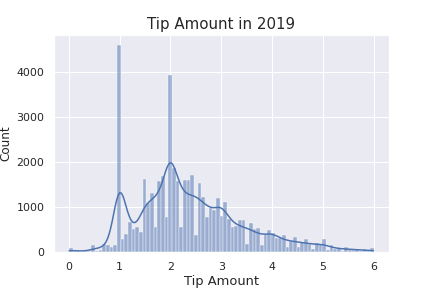
\includegraphics[width=0.8\linewidth]{Tip Amount in 2019.png}
   \end{minipage}\hfill
   \begin{minipage}{0.48\textwidth}
     \centering
     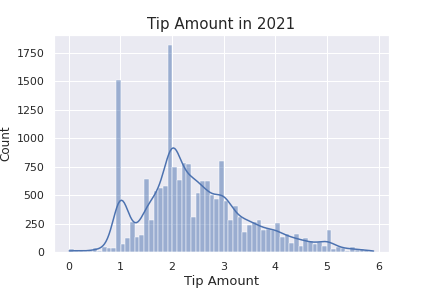
\includegraphics[width=0.8\linewidth]{Tip Amount in 2021.png}
   \end{minipage}
   \caption{Tip Amount in two years}
   \label{fig:1}
\end{figure}

\subsection{Numeric Features}
Selected Numeric features are: Trip Distance, Fare amount, Average Speed, Time Duration, Temperature and Wind Speed. Their correlations with the Tip Amount and Tip Rate are presented in Figure \ref{fig:2}. It implies that Tip Amount are relatively strong positively correlated to Trip Distance, Fare Amount and Time Duration, while Tip rate remains almost unaffected by all these features. However the Average Speed as a factor of the quality of a trip, should relate strong with passengers' satisfaction and the Tip amount, indeed shows up little correlation. A possible reason is that since we have unrealistic outliers removed, the Average Speed will generally fall into some reasonable region where most passengers won't feel strongly dissatisfied. Meanwhile the low correlations of Temperature and Wind Speed align with the expectation that weather details for a whole day could provide only limited support on prediction towards single trips.
\begin{figure}[h!]
    \centering
     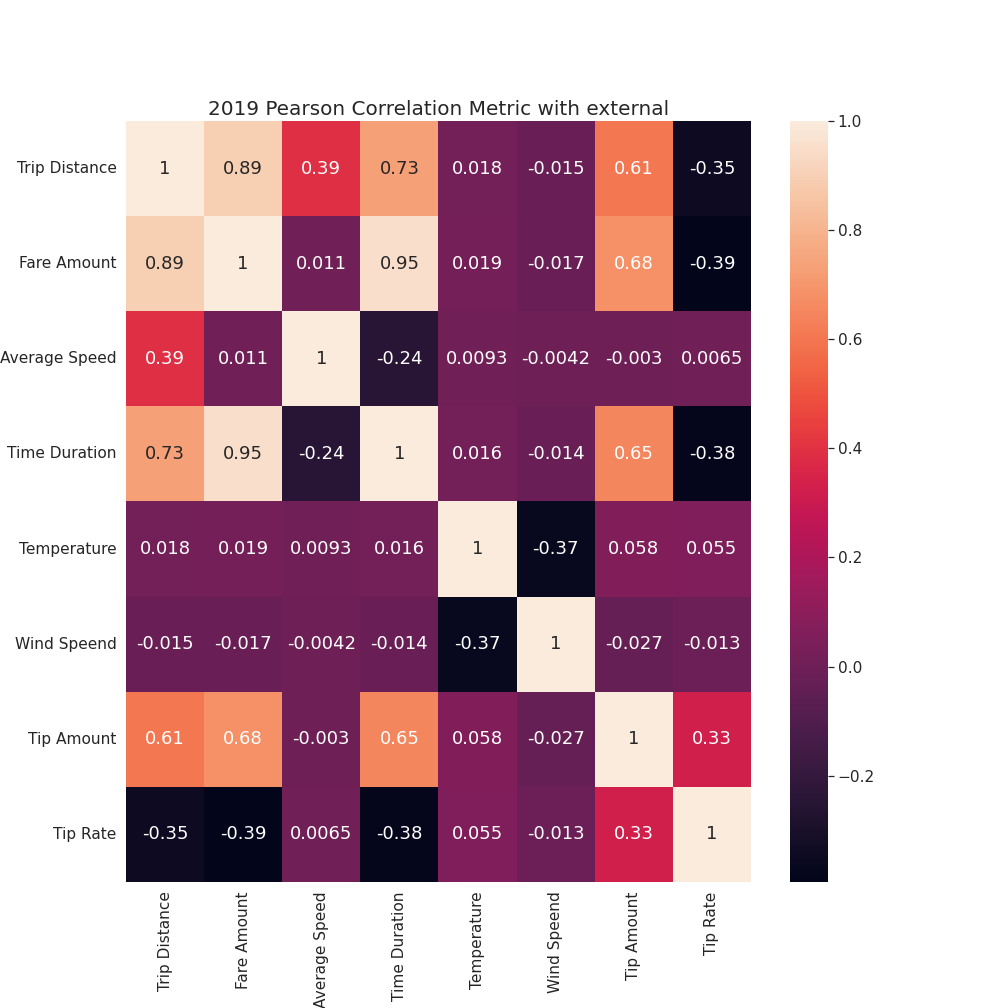
\includegraphics[width=0.6\linewidth, height = 0.5\linewidth]{2019 Pearson Correlation Metric with external.png}
   \caption{Numeric Features Correlation in 2019}
   \label{fig:2}
\end{figure}

\subsection{2019 vs 2021}
By comparing and contrasting the trend of the average tip amount and tip rate of each month in two years in Figure \ref{fig:3}, we aim to figure out people's Tip habit before and after COVID. For some reason, Jan 2019 demonstrates an exceptional low tipping which requires further investigation. Otherwise, two years shows up similar value and trend of tip amount throughout the year, with 2021 slightly higher towards the end of the year. This could be explained by the recovery of economic activities after the global pandemic such that people are more willing to pay tips. With the Tip rate, two years share almost exactly the same trend, with 2021 higher by 1\% which could be counted towards the general increasing purchasing power over the time. Based on such conclusion, predicting tip amount using previous years' data are reasonable and efficient. 
\begin{figure}[h!]
   \begin{minipage}{0.48\textwidth}
     \centering
     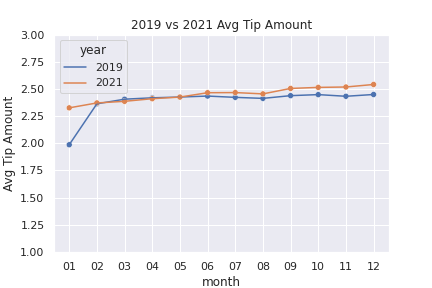
\includegraphics[width=1\linewidth]{2019 vs 2021 Avg Tip Amount.png}
   \end{minipage}\hfill
   \begin{minipage}{0.48\textwidth}
     \centering
     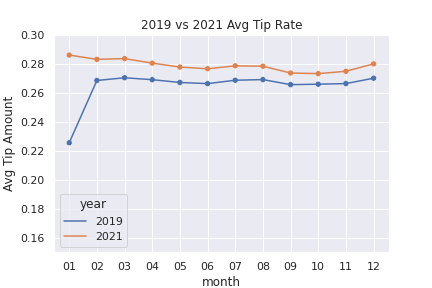
\includegraphics[width=1\linewidth]{2019 vs 2021 Avg Tip Rate.png}
   \end{minipage}
   \caption{Comparison between two years}
   \label{fig:3}
\end{figure}

\subsection{Categorical Features}
Three Categorical Features are explored: Is Weekend, Is Airport, Is Rainy. We take 2021-07 as the sample to see how are these affecting the tip habits in a certain month. Table \ref{table:3} demonstrates the average tip amount and rate under combinations of different categorical features. We see that the strongest feature pointing towards a high tip amount is 'Is Airport'. All trips that either Pick up or Drop off at the Airport will result into a larger Tip amount. However it produces lower Tip Rate since most trips relating to Airport often triggers a larger fare amount. Apart from that, higher tip rates will be paid on Weekdays. 'Is Rainy' demonstrates chaotic association.

\begin{table}[h!]
\centering
    \begin{tabular}{||c | c | c | c | c||}
    \hline
    Is Weekend & Is Airport & Is Rainy & Avg Tip Amount (\$) & Avg Tip Rate (\%)\\ [0.5ex] 
    \hline\hline
    \checkmark & $\times$ & $\times$ & 2.437 & 0.273\\ 
    \hline
    \checkmark & $\times$ & \checkmark & 2.440 & 0.275\\ 
    \hline
    \textcolor{blue}{$\times$} & $\times$ & \checkmark & 2.468 & \textcolor{blue}{0.280}\\ 
    \hline
    \textcolor{blue}{$\times$} & $\times$ & $\times$ & 2.474 & \textcolor{blue}{0.279}\\ 
    \hline
    \checkmark & \textcolor{red}{\checkmark} & $\times$ & \textcolor{red}{3.167} & 0.242\\ 
    \hline
    \checkmark & \textcolor{red}{\checkmark} & \checkmark & \textcolor{red}{3.194} & 0.248\\ 
    \hline
    \textcolor{blue}{$\times$} & \textcolor{red}{\checkmark} & \checkmark & \textcolor{red}{3.252} & \textcolor{blue}{0.247}\\ 
    \hline
    \textcolor{blue}{$\times$} & \textcolor{red}{\checkmark} & $\times$ & \textcolor{red}{3.265} & \textcolor{blue}{0.245}\\ 
    \hline
    
    
    \end{tabular}
\caption{Combinations of categorical features}
\label{table:3}
\end{table}

\subsection{Geospatial Analysis}
The Tip amount with respect to different Pick up location and Drop off location are plotted in Figure \ref{fig:4}. Clearly trips that are Dropped off in center districts of Queen and Brooklyn often triggers high tips of \$2.9 - \$3.4 which is definitely higher than the average level of \$2.3.
\begin{figure}[h!]
   \begin{minipage}{0.5\textwidth}
     \centering
     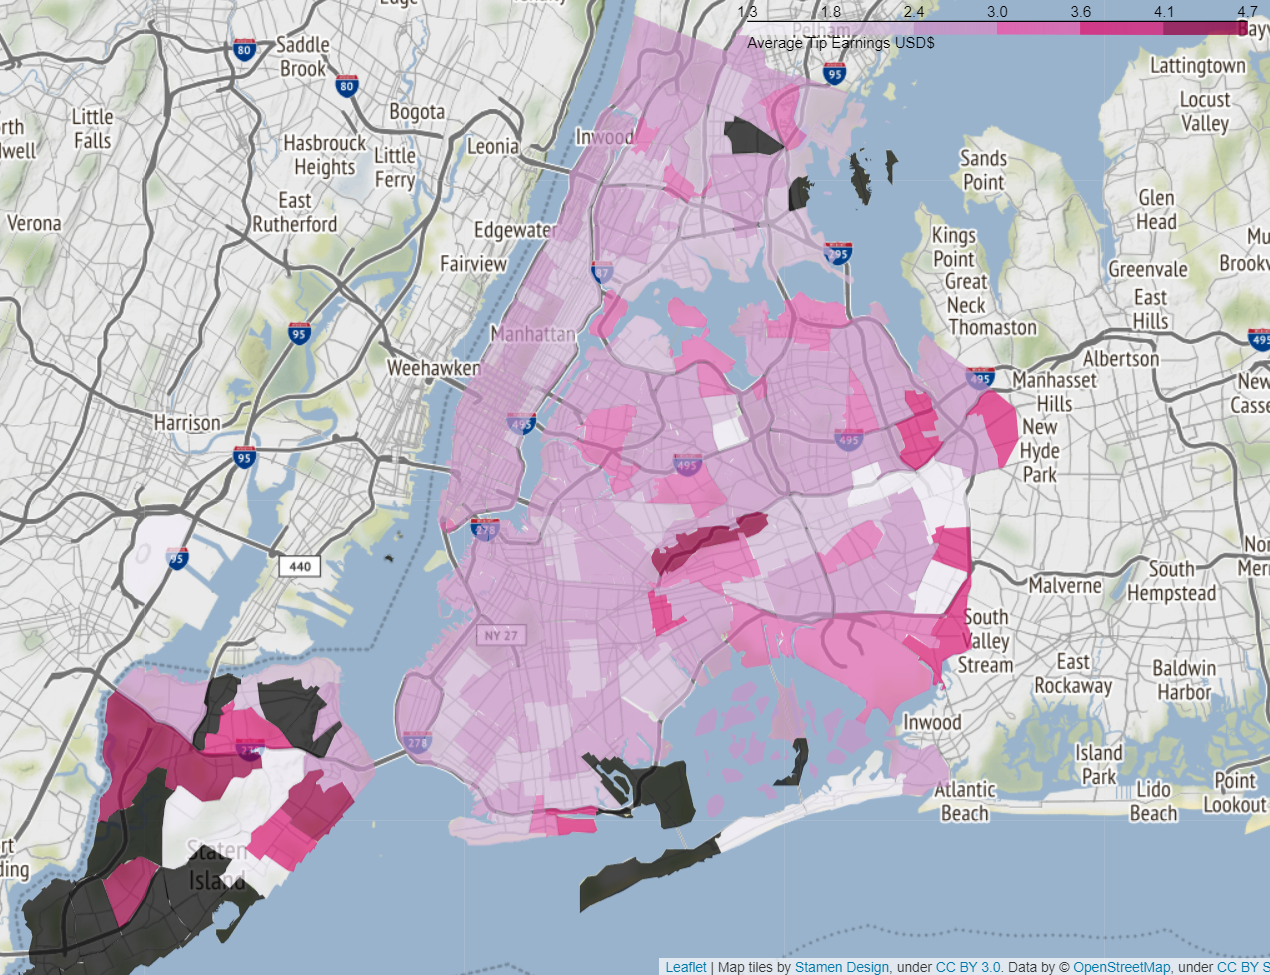
\includegraphics[width=0.8\linewidth]{PUmap.png}
   \end{minipage}\hfill
   \begin{minipage}{0.5\textwidth}
     \centering
     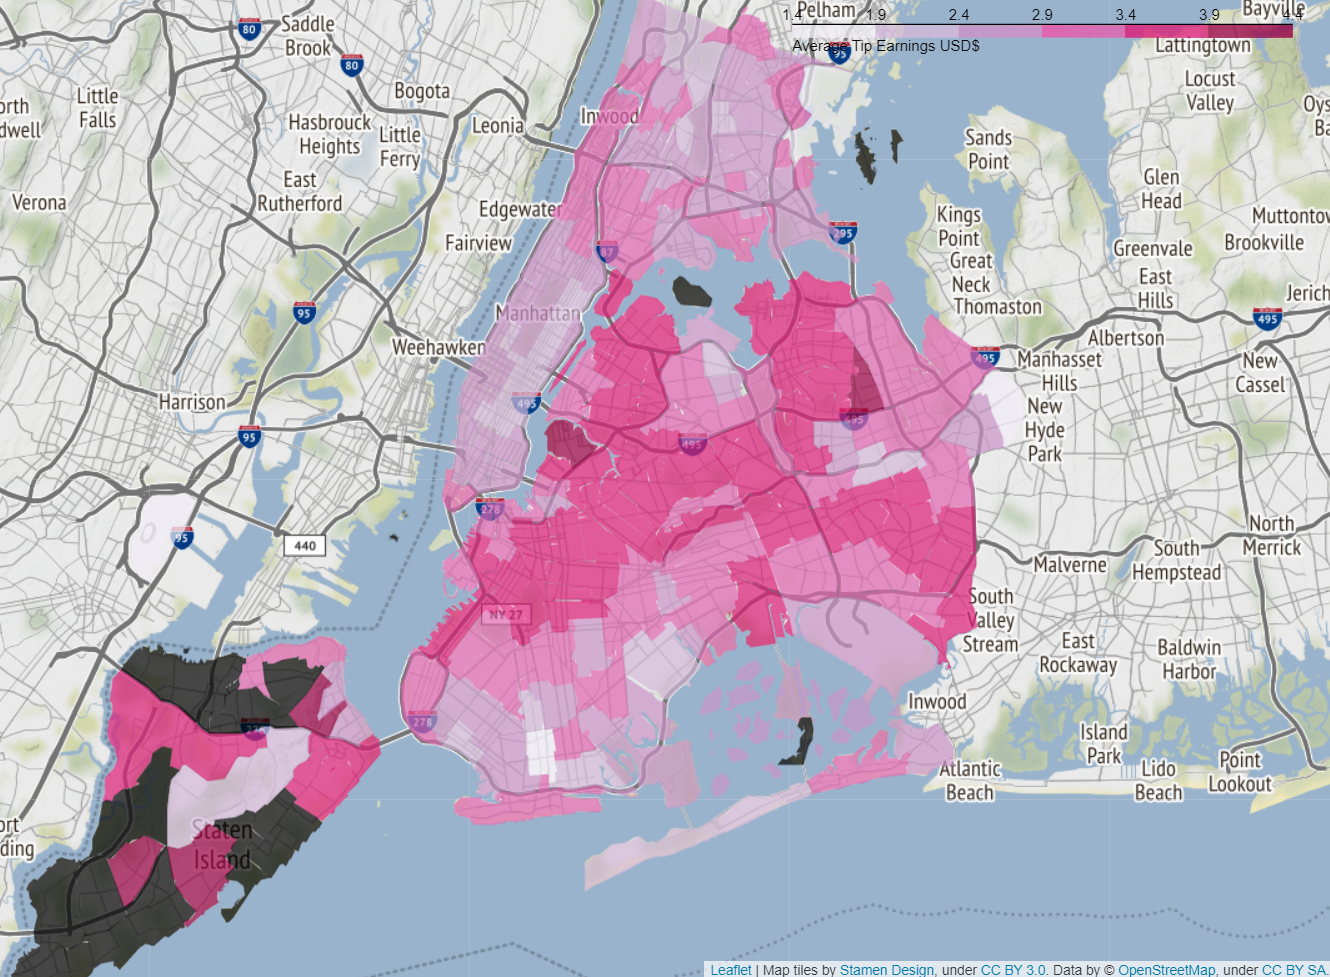
\includegraphics[width=0.8\linewidth]{DOmap.png}
   \end{minipage}
   \caption{Amount of Tip in different location}
   \label{fig:4}
\end{figure}


\section{Modelling}
Two models are introduced to deliver a comprehensive discussion towards the tip amount, with one model doing Regression and one doing Classification. Features passed in include 7 numeric attributes and 4 categorical attributes. The final response is focusing on the prediction of Tip Amount. The models are trained on Jun - Nov, 2021 and predicting Dec, 2021 since this timeline contains stable tip amount and tip rate.

\subsection{Random Forest Regressor (RFR)}
Random Forest Regressor\cite{5} is an ensemble regression model based on the idea of Random Forest: building multiple Decision Trees and combining them to take the average result as the final regression output. The bootstrapping methodology is also employed as each Decision Tree only takes part of the whole dataset to train. For each Decision Tree built, it will decide on the 'best split' attribute to cluster all instances, then keep iterating until the best result is produced. It is always outperforming on non-linear datasets due to such characteristics. Our final model contains 10 trees with each going to a maximum depth of 10.
\begin{figure}[h!]
     \centering
     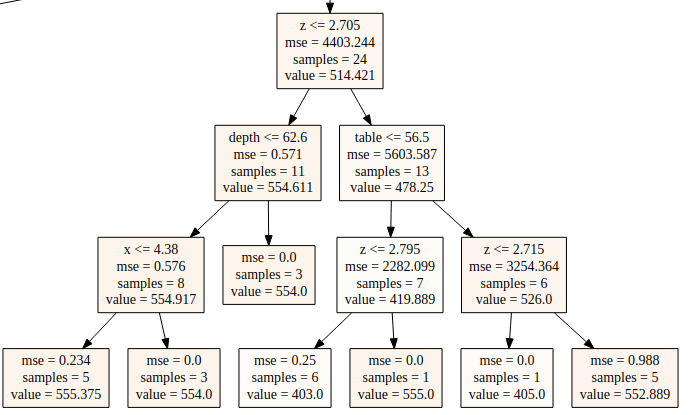
\includegraphics[width=0.5\linewidth]{RFR model.png}
   \caption{Demonstration of Random Forest Regressor}
   \label{fig:5}
\end{figure}



\subsubsection{Error Analysis}
Mean Squared Error (MSE) and Mean Absolute Error (MAE) are employed as the indicators of error analysis for RFR model as they directly measures the difference between prediction and actual result. With the comparison to the raw statistical variance of Tip amount, we aim to observe how much variation of the response variable could be explained by the model.

\begin{table}[h!]
\centering
    \begin{tabular}{||c  c || c  c  c|||}
    \hline
    & RFR model & Statistics & Test & Predictions\\
    \hline\hline
    MSE & 0.6041 & MEAN & \$2.5409 & \$2.5005\\
    MAE & 0.5333 & STD & 1.0193 & 0.6473\\
    \hline
    \end{tabular}
\caption{RFR model performance}
\label{table:4}
\end{table}

As shown in Table \ref{table:4}, the MSE and MAE are all at the level of 0.5, indicating the prediction accuracy towards the Tip amount is within 50 cents. Moreover, the model produces a prediction with almost the same mean value as the actual data while the standard deviation is almost halved. Such indicates a strong ability of the model to explain the ordinary Tip amount that are close to the fixed value with little ability to learn the extreme data. This also matches with the limitation of RFR model that no extrapolation could be carried out by the model since the splits done in the Trees based on the training data are not able to deal with unseen values.

Same results could be achieved by observing the two plots in Figure \ref{fig:6}. The distribution of residuals approximately follows a Gaussian Distribution which gathers strongly around 0, demonstrating a generally good performance. Further more, the prediction follows the Normal QQ-plot well in the centering region while shows up deviation towards the tails. An over-estimation is observed towards the right end and an under-estimation is observed towards the left end. This aligns with the previous analysis that the model learns the general Tip amount well, whereas performs poor towards extreme values.

\begin{figure}[h!]
   \begin{minipage}{0.5\textwidth}
     \centering
     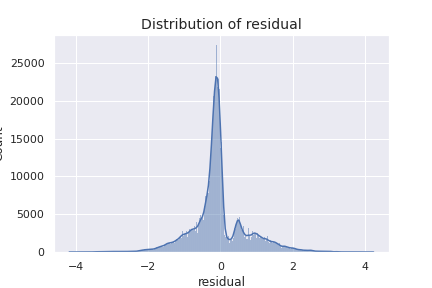
\includegraphics[width=\linewidth, height = 5cm]{Distribution of residual.png}
   \end{minipage}\hfill
   \begin{minipage}{0.5\textwidth}
     \centering
     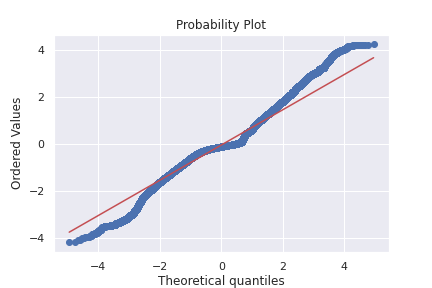
\includegraphics[width=\linewidth, height = 5cm]{QQ plot.png}
   \end{minipage}
   \caption{Plots for Error analysis}
   \label{fig:6}
\end{figure}


\subsection{Logistic Regression (LR)}
A further focus on the extreme Tip amount, especially those that are large, will be delivered as a binary classification task. All Tip amount are separated into two classes: those greater than \$2 are considered as High Tip and the rest are considered as Low Tip. Since \$2 is assumed to be a recommended Tip amount provided to the passengers as analysed in section 3.1, we aim to focus on the trips that pay a higher value than the recommended therefore adopted \$2 as a boundary. The Logistic Regression model is built upon binary family and the Elastic Net parameter is taken as 1.


\subsubsection{Error Analysis}
Accuracy, Recall, Precision and F1 score are employed to evaluate the model performance. Confusion matrix is not included since the counts of trips are too large. From Table \ref{table:5}, a high Accuracy and Recall is observed demonstrating the model's power to capture the characteristics of those trips with high Tip amount. Meanwhile the high F1 score implies the balance between the model's unbiased learning towards both High and Low Tip amount.
\begin{table}[h!]
\centering
    \begin{tabular}{||c  c  c  c | c ||}
    \hline
    Accuracy & Recall & Precision & F1 score & baseline\\
    \hline\hline
    0.7619 & 0.8640 & 0.7890 & 0.8248 & 0.6311\\
    \hline
    \end{tabular}
\caption{Logistic Regression Model performance}
\label{table:5}
\end{table}


\subsection{Discussion}
Both models demonstrates a strong ability in dealing with the mixture of both categorical and numeric features, which definitely outperforms most of the other statistical models for this task. The RFR model works in a way that categorical features are designed for clustering stage while the numeric features are informative towards the final prediction. Meanwhile, the RFR model includes the sufficient weighting criteria at the nodes of each tree and similar concept is showcased in the LR model by assigning different weights to the features passed in. Thus both models require little manual feature selection. 

The RFR model aims for precise prediction which is proven to work well with conventional Tip amount. However it is not that sensitive to predict extreme Tip amount. To achieve a further level of Tip analysis, the classification LR model is adopted. The final high Recall and F1 score demonstrates its strength at learning the true characteristics of the trips with a higher Tip amount. Thus a better identification on the Tips could be reached with the combination of the two models as they complements each other. An advanced ensemble method could be established based on these two in further study. We could train several RFR models each for predicting a certain level of Tip amount and then using prediction label from LR model to indicate which RFR model should be weighed the most.

However a huge disadvantage of RFR model is that it performs like a `black box' with little interpretability. Same goes with LR model as the algorithm only works on figuring the boundary of low and high Tips, without detailed elaboration on the exact effect of each feature.



\section{Conclusion}
To conclude this research, we recommend the taxi provider companies to construct a similar model with advanced features and data put into. Dataset with more details and precision could be employed such that more deeper characteristics of each attribute could be exposed. This analyse towards Tips provides the companies an alternative way to check the quality of services they provide in addition to direct feedback from the passengers. 

Now assuming the perspective of the drivers, one specific recommendation seen from Figure \ref{fig:3} is that the best time to earn more tips will be at the start and end of the year, probably over the Christmas ad New Year's period when pleasant travelling trips increases. More generally, the improved model could advise the drivers on more profitable trips and trigger a stronger willing to provide better services as they are potentially earning more without explicit personal effort. In general, a detailed investigation on Tips provides both the taxi service owner and provider a chance to comprehensively learn about their own business from a side way.

The largest limitation of this study is the lack of computing power such that most analysis aims to provide a clear indication of direction. To further improve the results, we recommend more relevant datasets with precise attribute values being adopted. In addition, the Tip behaviour of those passengers who pay by cash are likely to be completely different and thus waiting for investigation. More interpretable models are also encouraged to be addressed to conduct detailed analysis on the influential factors.



\clearpage

% BEGIN REFERENCES SECTION
\printbibliography

\end{document}